\documentclass[xcolor={table}]{beamer}
\usepackage{fleqn}
\usepackage{graphicx}
\usepackage{coordsys} %for \numbline commander

%Setup appearance:
\usetheme{Darmstadt}
\usefonttheme[onlylarge]{structurebold}
\setbeamerfont*{frametitle}{size=\normalsize,series=\bfseries}
\setbeamertemplate{navigation symbols}{}
\setbeamertemplate{bibliography item}{[\theenumiv]}

% Standard packages
\usepackage[english]{babel}
\usepackage[latin1]{inputenc}
\usepackage{times}
\usepackage[T1]{fontenc}
\usepackage{multirow}
\usepackage{subfigure}
\usepackage{pbox}
\usepackage{arydshln}
\usepackage{pifont}
\usepackage{cancel}
\usepackage{rotating} % for sideways headings

% Source Code packages
\usepackage{algorithm2e}
\usepackage{algorithmic}

\DeclareSymbolFont{extraup}{U}{zavm}{m}{n}
\DeclareMathSymbol{\varclub}{\mathalpha}{extraup}{84}
\DeclareMathSymbol{\varspade}{\mathalpha}{extraup}{85}
\DeclareMathSymbol{\varheart}{\mathalpha}{extraup}{86}
\DeclareMathSymbol{\vardiamond}{\mathalpha}{extraup}{87}

%%% This section command that adds a big page with section dividers
\usepackage{xifthen}% provides \isempty test
\newcommand{\SectionSlide}[2][]{
	\ifthenelse{\isempty{#1}}
		{\section{#2}\begin{frame} \begin{center}\begin{huge}#2\end{huge}\end{center}\end{frame}}
		{\section[#1]{#2}\begin{frame} \begin{center}\begin{huge}#2\end{huge}\end{center}\end{frame}}
}
%Extends the section slide to to include a shortened section title for the navigation bar as a second parameter
\newcommand{\SectionSlideShortHeader}[3][]{
	\ifthenelse{\isempty{#1}}
		{\section[#3]{#2}\begin{frame} \begin{center}\begin{huge}#2\end{huge}\end{center}\end{frame}}
		{\section[#1]{#2}\begin{frame} \begin{center}\begin{huge}#3\end{huge}\end{center}\end{frame}}
}

\newcommand{\refer}[1]{\footnote{#1}}
\newcommand{\GW}{\text{\textit{Guess-Who~}}}
\newcommand{\keyword}[1]{\alert{\textbf{#1}}\index{#1}}
\newcommand{\firstkeyword}[1]{\textbf{#1}\index{#1}}
\newcommand{\indexkeyword}[1]{\alert{\textbf{#1}\index{#1}}}
\newcommand{\featN}[1]{\textsc{#1}}
\newcommand{\featL}[1]{\textit{'#1'}}
 \newcommand{\ourRef}[1]{\ref{#1} $^{\text{\tiny[\pageref{#1}]}}$}
 \newcommand{\ourEqRef}[1]{\eqref{#1}$^{\text{\tiny[\pageref{#1}]}}$}
  
\DeclareMathOperator*{\argmax}{argmax}
\DeclareMathOperator*{\argmin}{argmin}

\title{Appendix C Differentiation Techniques\\for Machine Learning}
	\author{John D. Kelleher and Brian Mac Namee and Aoife D'Arcy}
	\institute{}
	\date{}

\begin{document}
\begin{frame}
	\titlepage
\end{frame}
\begin{frame}
	 \tableofcontents
\end{frame}

\section{Basic Concepts}

 \begin{frame} [plain]
Imagine a car journey where we start out driving on a minor road at about $30$mph and then move onto a highway where we drive at about $80$mph before noticing an accident and braking suddenly.
\begin{figure}[hbt]
\begin{center}
\subfigure[]{\label{fig:derivSpeed}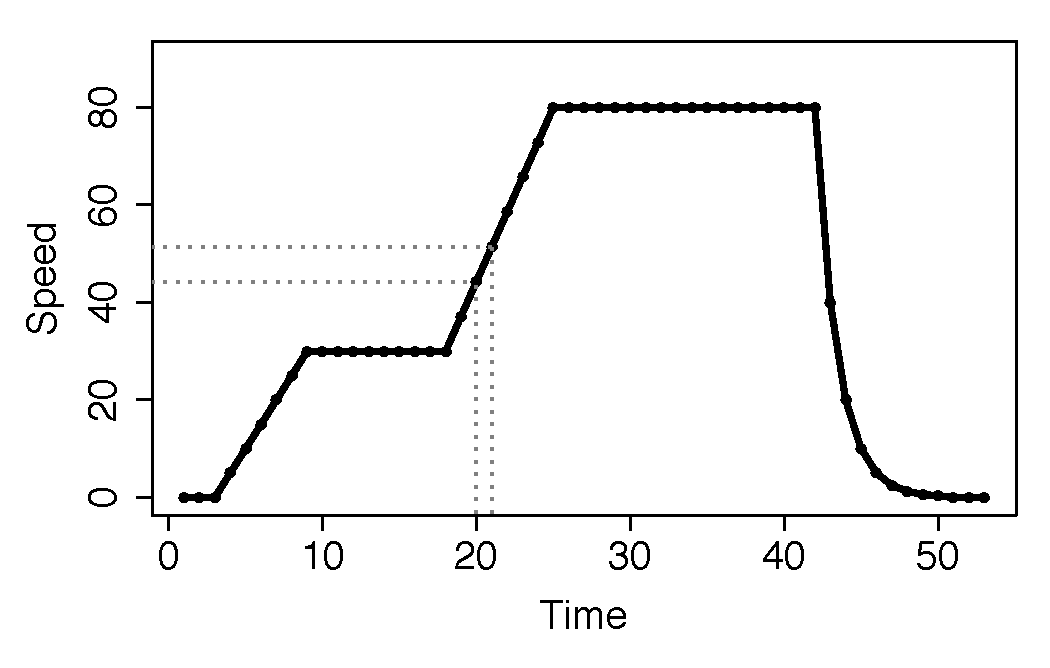
\includegraphics[width=0.40\textwidth]{./images/derivativesExampleSpeedGraph.pdf}}
\subfigure[]{\label{fig:derivAcceleration}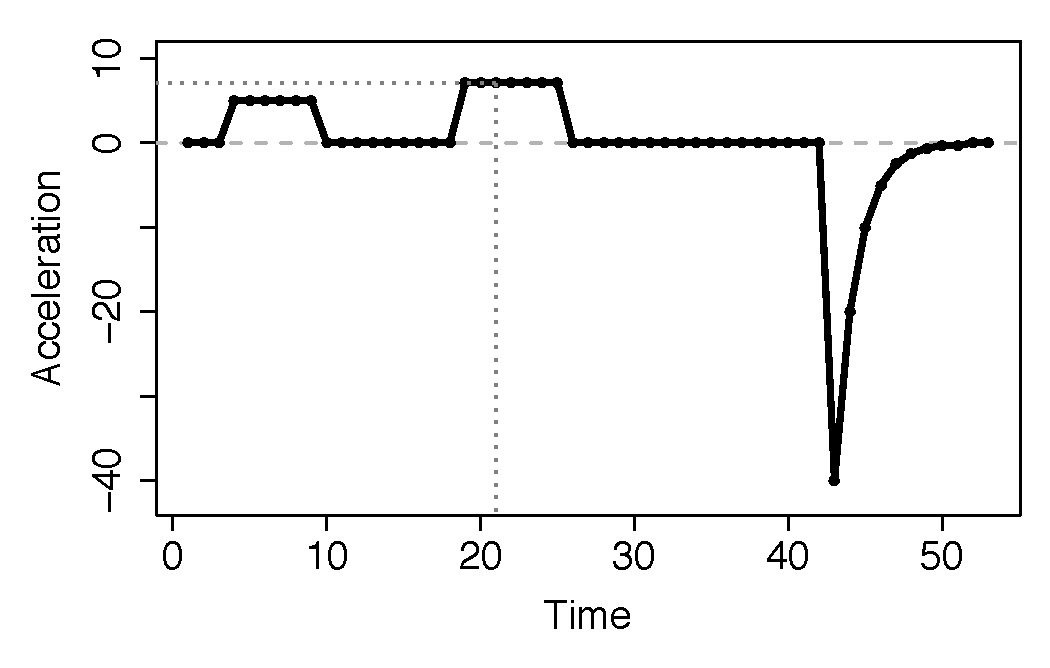
\includegraphics[width=0.40\textwidth]{./images/derivativesExampleAccelerationGraph.pdf}}
\caption{(a) the speed of a car during a journey along on the minor road before joining a motorway and finally coming to a sudden (safe) halt. (b) shows acceleration, the derivative of speed with respect to time, during this journey.}
\label{fig:derivSpeedAcceleration}
\end{center}
\end{figure}
\end{frame} 

\begin{frame} 
\begin{itemize}
\item Acceleration is a measure of the rate of change of speed over time. 
\item We can say more formally that acceleration is, in fact, the \keyword{derivative} of speed \textit{with respect to} time. 
\item \keyword{Differentiation} is the set of techniques from \keyword{calculus} (the branch of mathematics that deals with how things change) that allows us to calculate \keyword{derivatives}.
\end{itemize}
\end{frame} 

\section{Derivatives of Continuous Functions}

 \begin{frame} 
\begin{itemize}
\item  A \keyword{continuous function}, $f(x)$, generates an output for every value of a variable $x$ based on some expression involving $x$. For example:
 \begin{eqnarray*}
f(x) & = & 2x + 3 \\
f(x) & = & x^2 \\
f(x) & = & 3x^3 + 2x^2 - x - 2
\end{eqnarray*}
\item The first function is known as a \keyword{linear function} as the output is a combination of only additions and multiplications
\item The other two functions are known as \keyword{polynomial functions} as they include addition, multiplication and raising to exponents (we show a \keyword{second order polynomial function}, also known as a \keyword{quadratic function} and a \keyword{third order polynomial function}, also known as \keyword{cubic function}.
\end{itemize}
\end{frame} 



 \begin{frame} [plain]
\begin{figure}[!htb]
\begin{center}
\subfigure[$f(x) = 2x + 3 $]{\label{fig:derivExample1}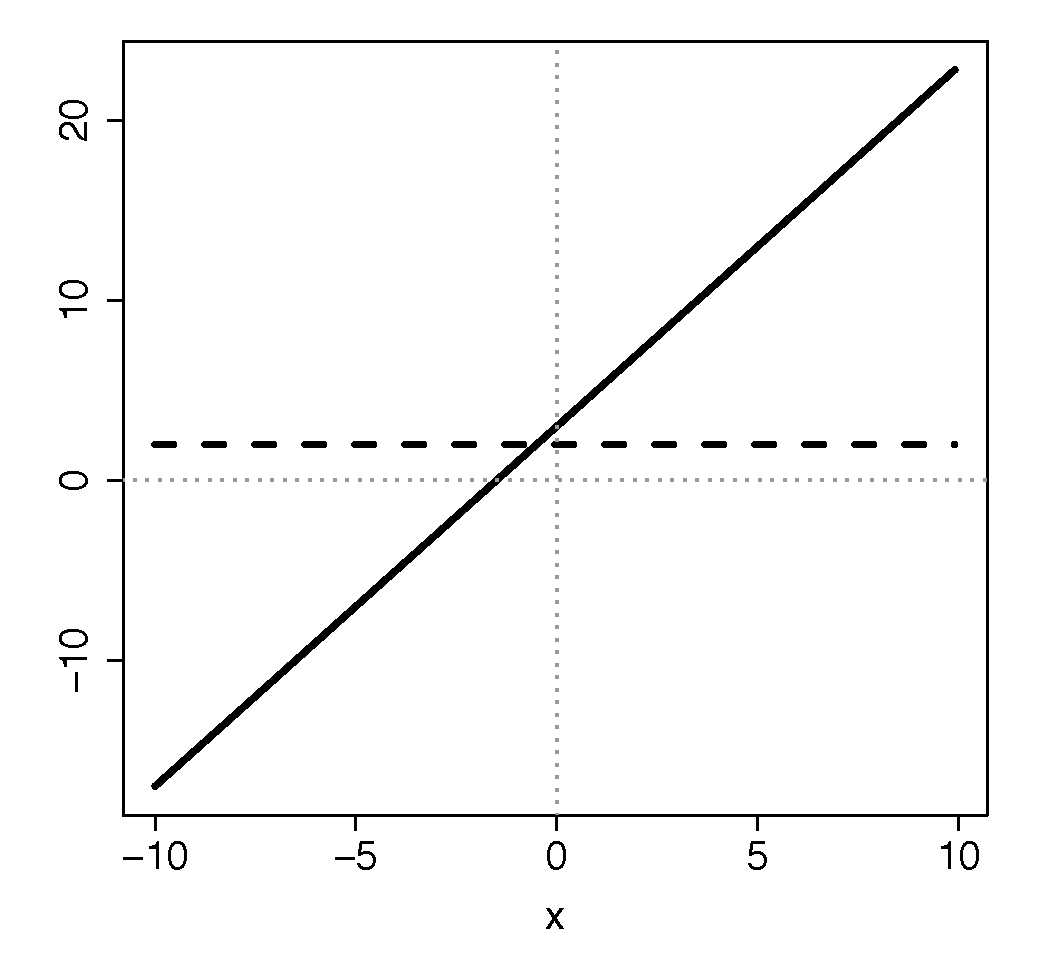
\includegraphics[width=0.49\textwidth]{./images/derivativesExamples1.pdf}}
\subfigure[$f(x) = x^2 $]{\label{fig:derivExample2}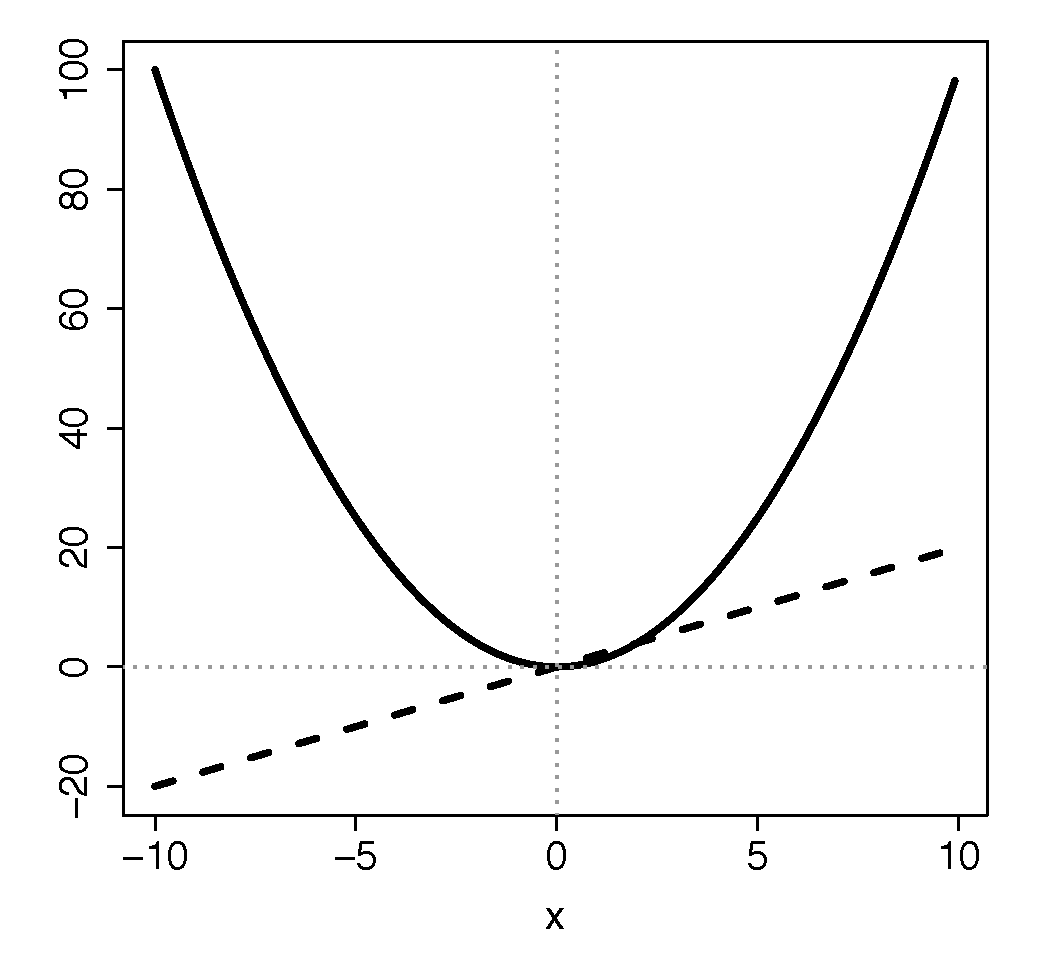
\includegraphics[width=0.49\textwidth]{./images/derivativesExamples2.pdf}}
\caption{(a) - (b) Some examples of continuous functions, shown as solid lines, and their derivatives, shown as dashed lines. }
\label{fig:derivExample}
\end{center}
\end{figure}
\end{frame} 

\begin{frame} 
\begin{alertblock}{Derivatives and Slopes!}
\begin{itemize}
	\item The derivative of a function $f(x)$ with respect to $x$ also gives us the slope of the function at that value of $x$.
\end{itemize}
\end{alertblock}
\end{frame}

\begin{frame} 
\begin{itemize}
\item To actually calculate the derivative, referred to as $\frac{d}{dx}f(x)$, of a simple continuous function, $f(x)$, we use a small number of differentiation rules:
\end{itemize}
\begin{center}
{\renewcommand{\arraystretch}{2}\begin{tabular}{r l c l l }
1) & $\displaystyle\frac{d}{dx} \alpha  $ & $= $ & $0$ & \parbox{6.5cm}{(where $\alpha$ is any constant)} \\
2) & $\displaystyle\frac{d}{dx} \alpha x^n  $ & $  = $ & $\alpha \times n \times x^{n - 1}$ &   \\
3) & $\displaystyle\frac{d}{dx} a + b  $ & $ = $ & $\displaystyle\frac{d}{dx}a + \displaystyle\frac{d}{dx} b$ &  \parbox{5cm}{(where $a$ and $b$ are expressions that may or may not contain $x$)} \\
4) & $\frac{d}{dx} \alpha \times c $ & $ = $ & $\alpha \times \displaystyle\frac{d}{dx} c$ &   \parbox{5cm}{(where $\alpha$ is any constant and $c$ is an expression containing $x$)}
\end{tabular}}
\end{center}
\end{frame} 

\section{The Chain Rule}

\begin{frame} 
\begin{itemize}
\item The function $f(x) = (x^2+1)^2$ cannot be differentiated using the rules just described because it is a \keyword{composite function} - it is a \textit{function of a function}. 
\end{itemize}
\begin{figure}[!htb]
\begin{center}
\subfigure[$f(x) = (x^2+1)^2$ ]{\label{fig:chainRuleExample1}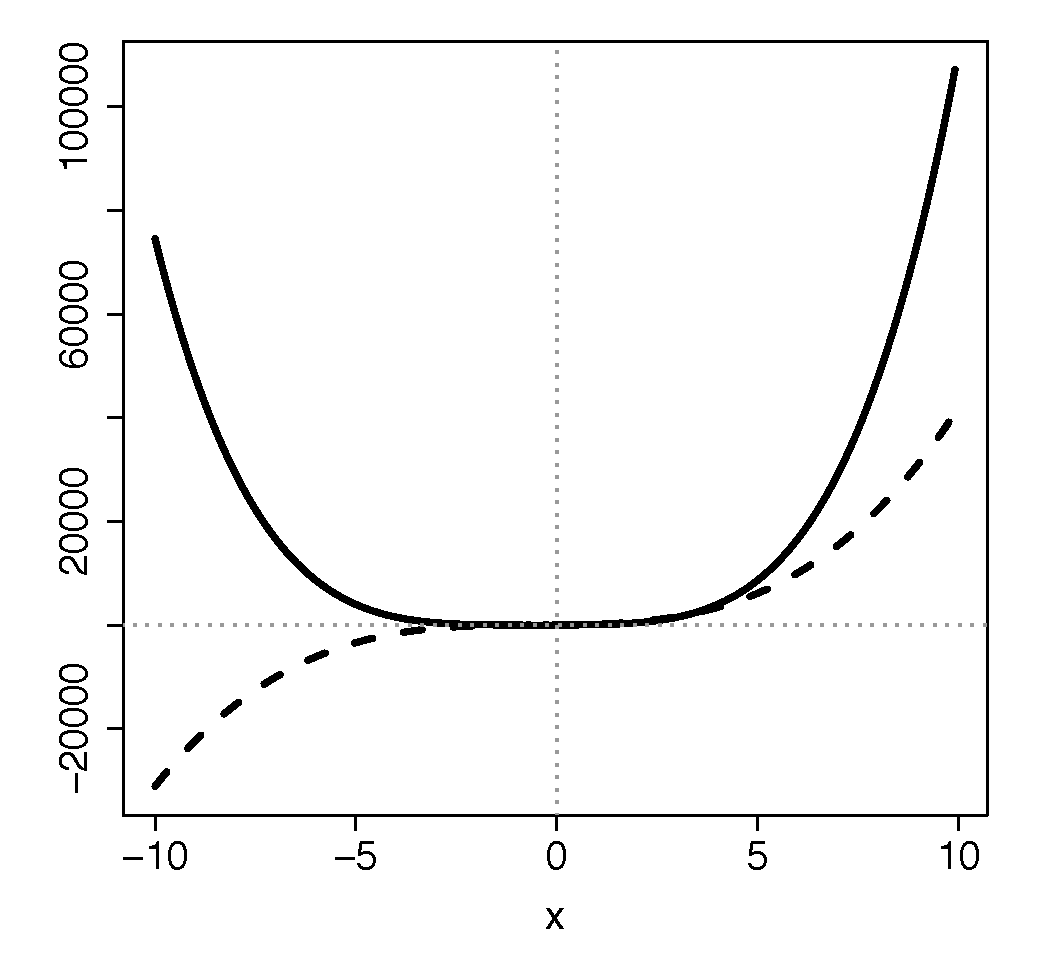
\includegraphics[width=0.45\textwidth]{./images/derivativesExamples5.pdf}}
\caption{A composite function and it's derivative.}
\label{fig:derivExample}
\end{center}
\end{figure}
\end{frame} 

\begin{frame} 
\begin{itemize}
\item We can rewrite $f(x)$ as $f(x) = \left(g\left(x\right)\right)^2$ where $g(x) = x^2+1$. 
\item The differentiation \alert{chain rule} allows us to differentiate functions of this kind of function.
\end{itemize}
	\begin{alertblock}{The Chain Rule}
\begin{equation}
\frac{d }{d x} f\left(g\left(x\right)\right) = \frac{d}{d~g(x)} f\left(g\left(x\right)\right) \times \frac{d }{d x} g\left(x\right)
\end{equation}
\end{alertblock}
\end{frame}

\begin{frame} 
\begin{itemize}
\item Applying this to the example $f(x) = (x^2+1)^2$ we get:
\begin{eqnarray*}
\displaystyle \frac{d }{d x} (x^2+1)^2 & = & \displaystyle \frac{d}{d~(x^2 + 1)} (x^2+1)^2 \times \displaystyle \frac{d }{d x} (x^2+1) \\
	&	= & \left(2 \times (x^2 + 1) \right) \times \left(2x\right) \\
	&	= & 4x^3  + 4x
\end{eqnarray*}
\end{itemize}
\end{frame} 

\section{Partial Derivatives}

\begin{frame} 
\begin{itemize}
\item Some functions are not defined in terms of just one variable. 
\item For example, $f(x, y) = x^2 - y^2 + 2x + 4y - xy + 2$ is a function defined in terms of two variables $x$ and $y$. 
\item Rather than defining a curve (as was the case for all of the previous examples) this function defines a surface. 
\end{itemize}
\end{frame} 

\begin{frame} [plain]
\begin{figure}[htb]
\begin{center}
\subfigure[$f(x, y) = x^2 - y^2 + 2x + 4y - xy + 2 $]{\label{fig:partialDerivExample1}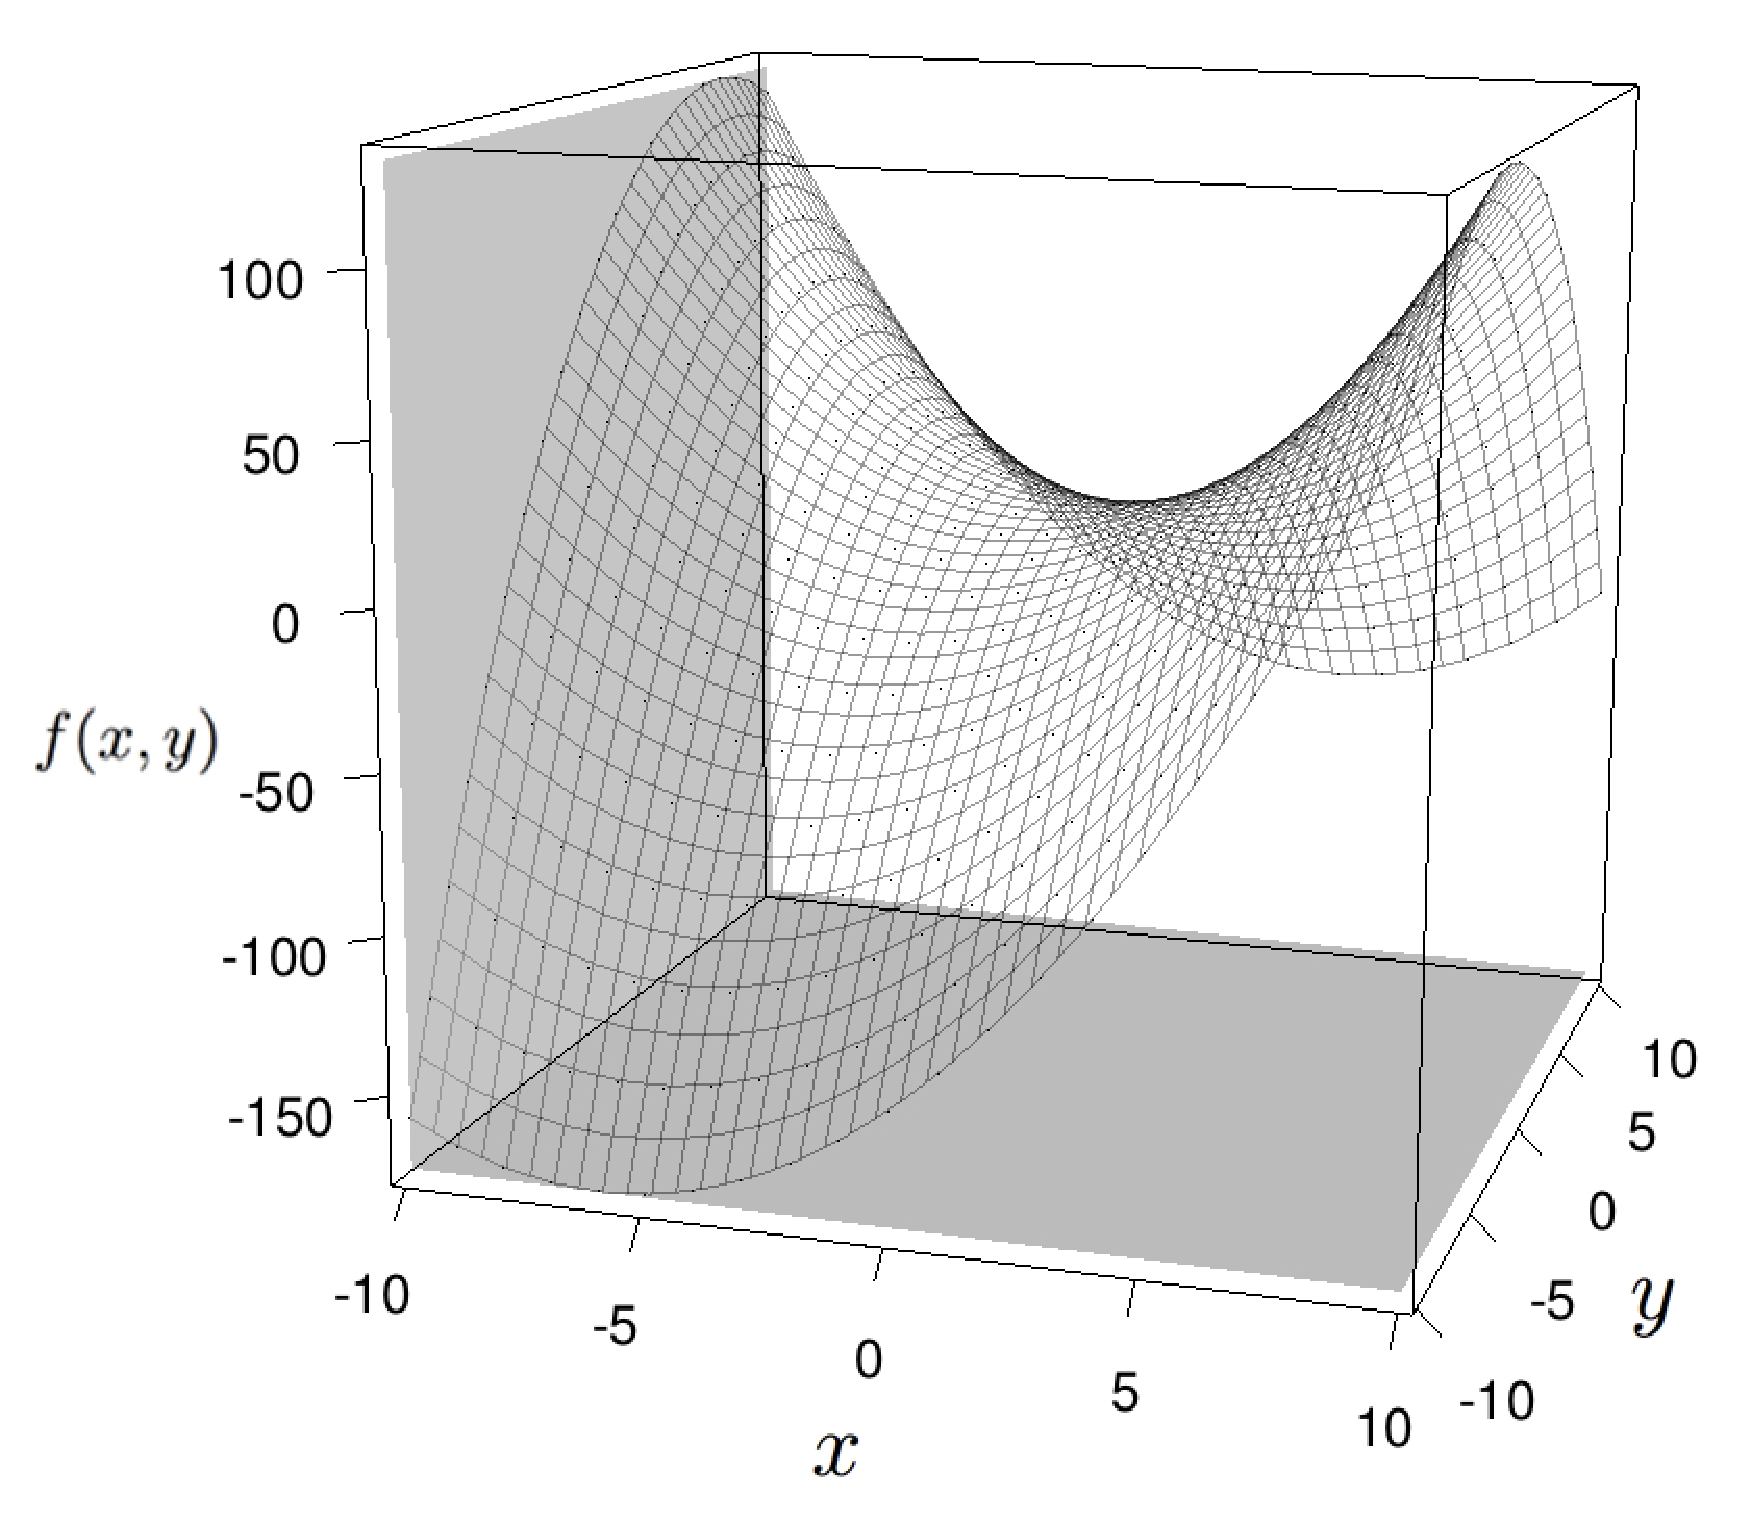
\includegraphics[width=0.75\textwidth]{./images/PartialDerivativesExampleFull.pdf}}
\caption{A continuous function in two variables, $x$ and $y$.}
\label{fig:partialDerivExample}
\end{center}
\end{figure}
\end{frame} 


\begin{frame} 
\begin{itemize}
\item Using \keyword{partial derivatives} offers us an easy way to calculate the derivative of a function like this. 
\item A partial derivative (denoted by the symbol $\partial$) of a function of more than one variable is its derivative with respect to one of those variables with the other variables held constant.
\end{itemize}
\end{frame} 

\begin{frame} 
\begin{itemize}
\item For the example function $f(x, y) = x^2 - y^2 + 2x + 4y - xy + 2$ we get two partial derivatives:
\begin{eqnarray*}
\frac{\partial}{\partial x}(x^2 - y^2 + 2x + 4y  - xy + 2) & = & 2x + 2 - y
\end{eqnarray*}
\noindent where the terms $y^2$ and $4y$ are treated as constants as they do not include $x$, and: 
\begin{eqnarray*}
\frac{\partial}{\partial y}(x^2 - y^2 + 2x + 4y - xy + 2) = -2y + 4 - x
\end{eqnarray*}
\noindent where the terms $x^2$ and $2x$ are treated as constants as they do not include $y$. Figures \ourRef{fig:partialDerivExample2} and \ourRef{fig:partialDerivExample3} show these partial derivatives. 
\end{itemize}
\end{frame} 

 \begin{frame} 
\begin{figure}[htb]
\begin{center}
\subfigure[$f(x, y) = x^2 - y^2 + 2x + 4y - xy + 2 $]{\label{fig:partialDerivExample1}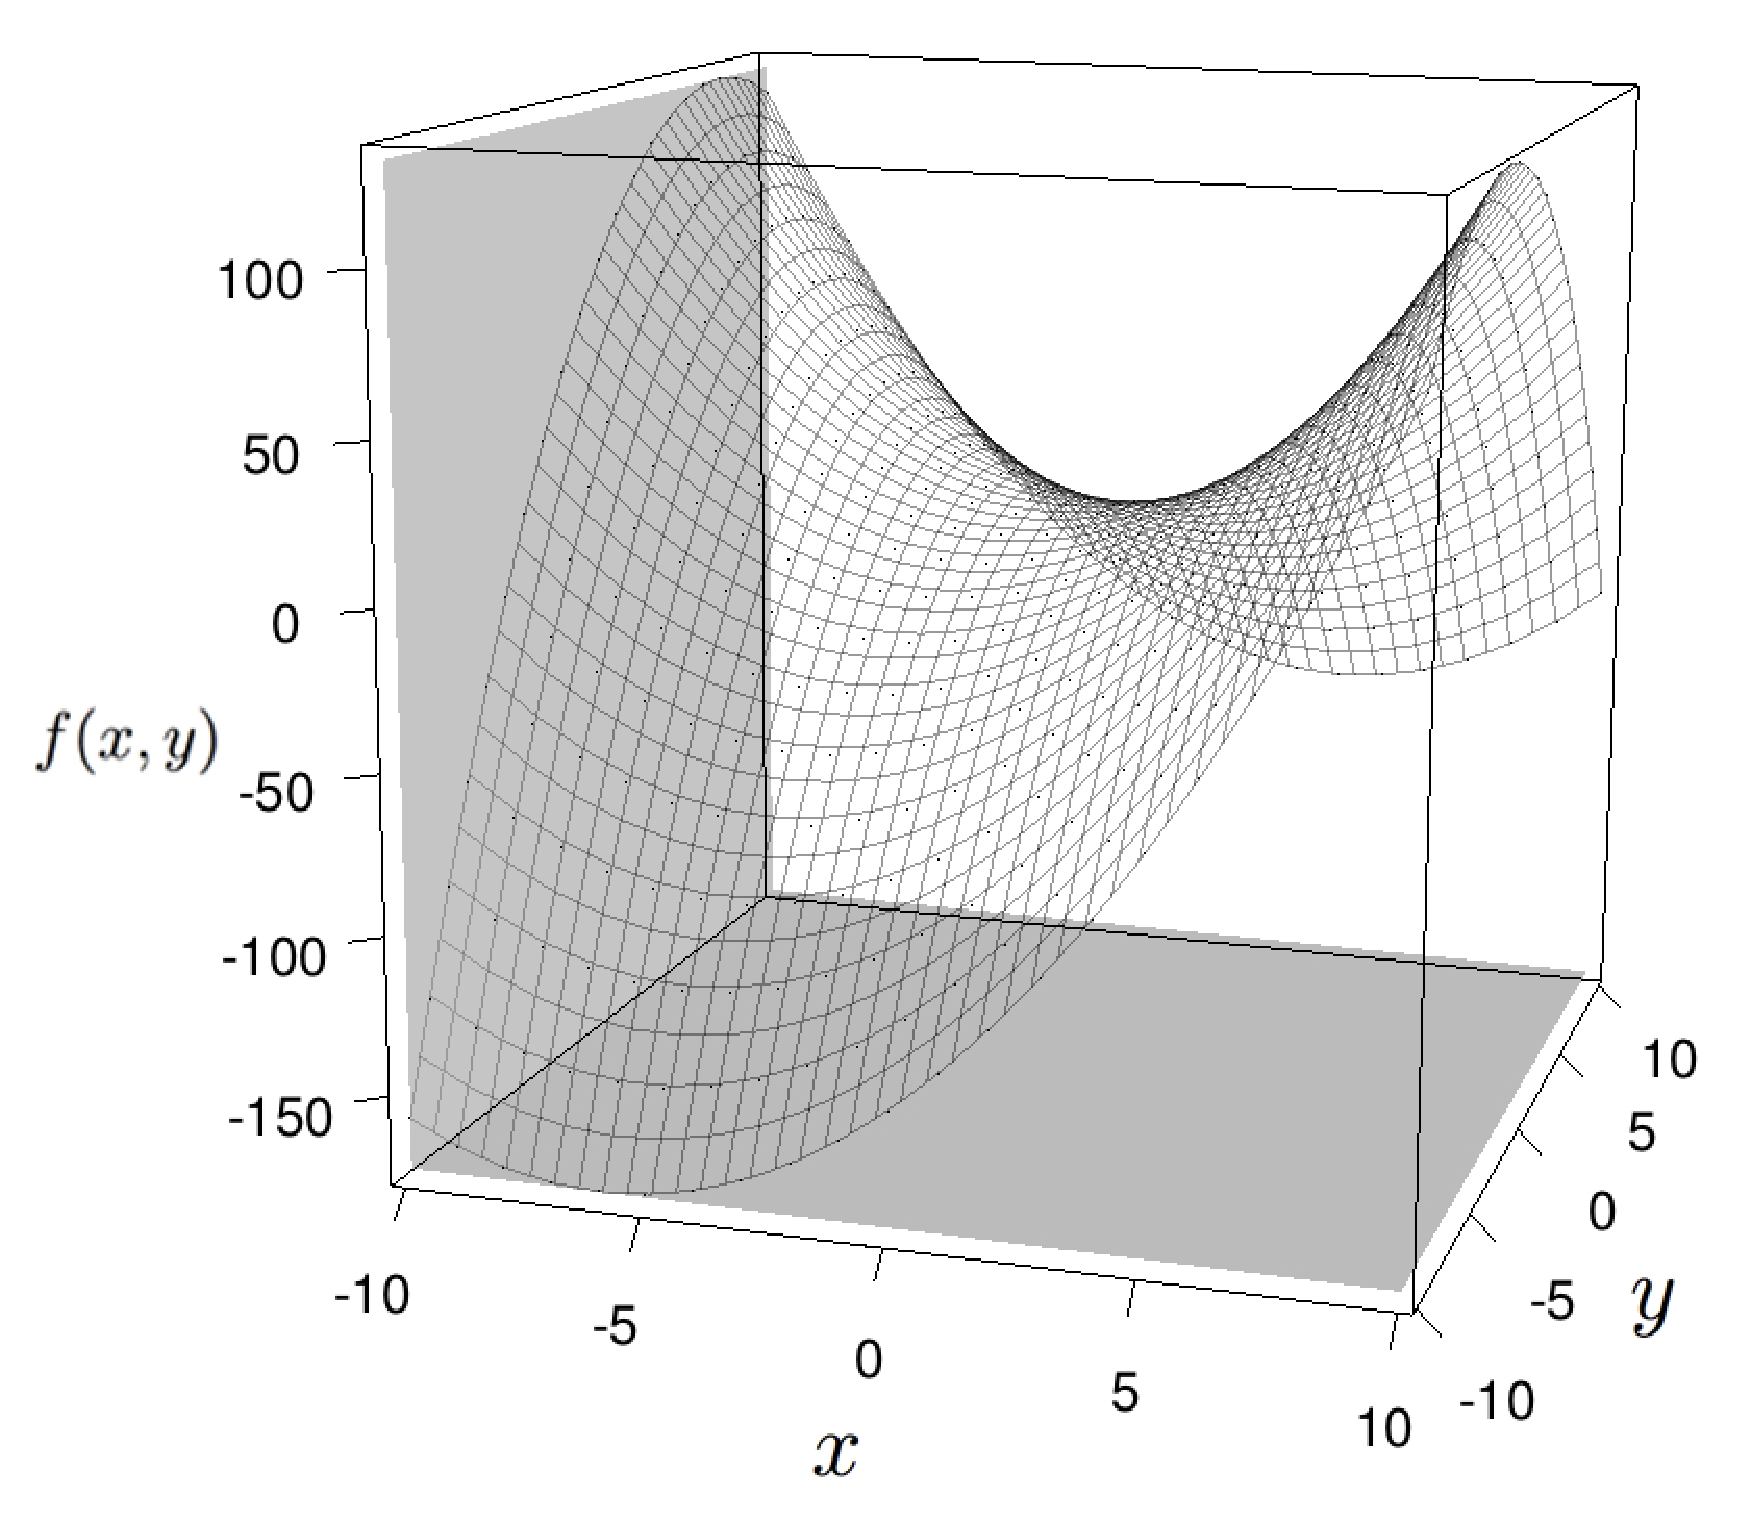
\includegraphics[width=0.32\textwidth]{./images/PartialDerivativesExampleFull.pdf}}
\subfigure[$\displaystyle \frac{\partial}{\partial x} f(x, y) = 2x + 2 - y$]{\label{fig:partialDerivExample2}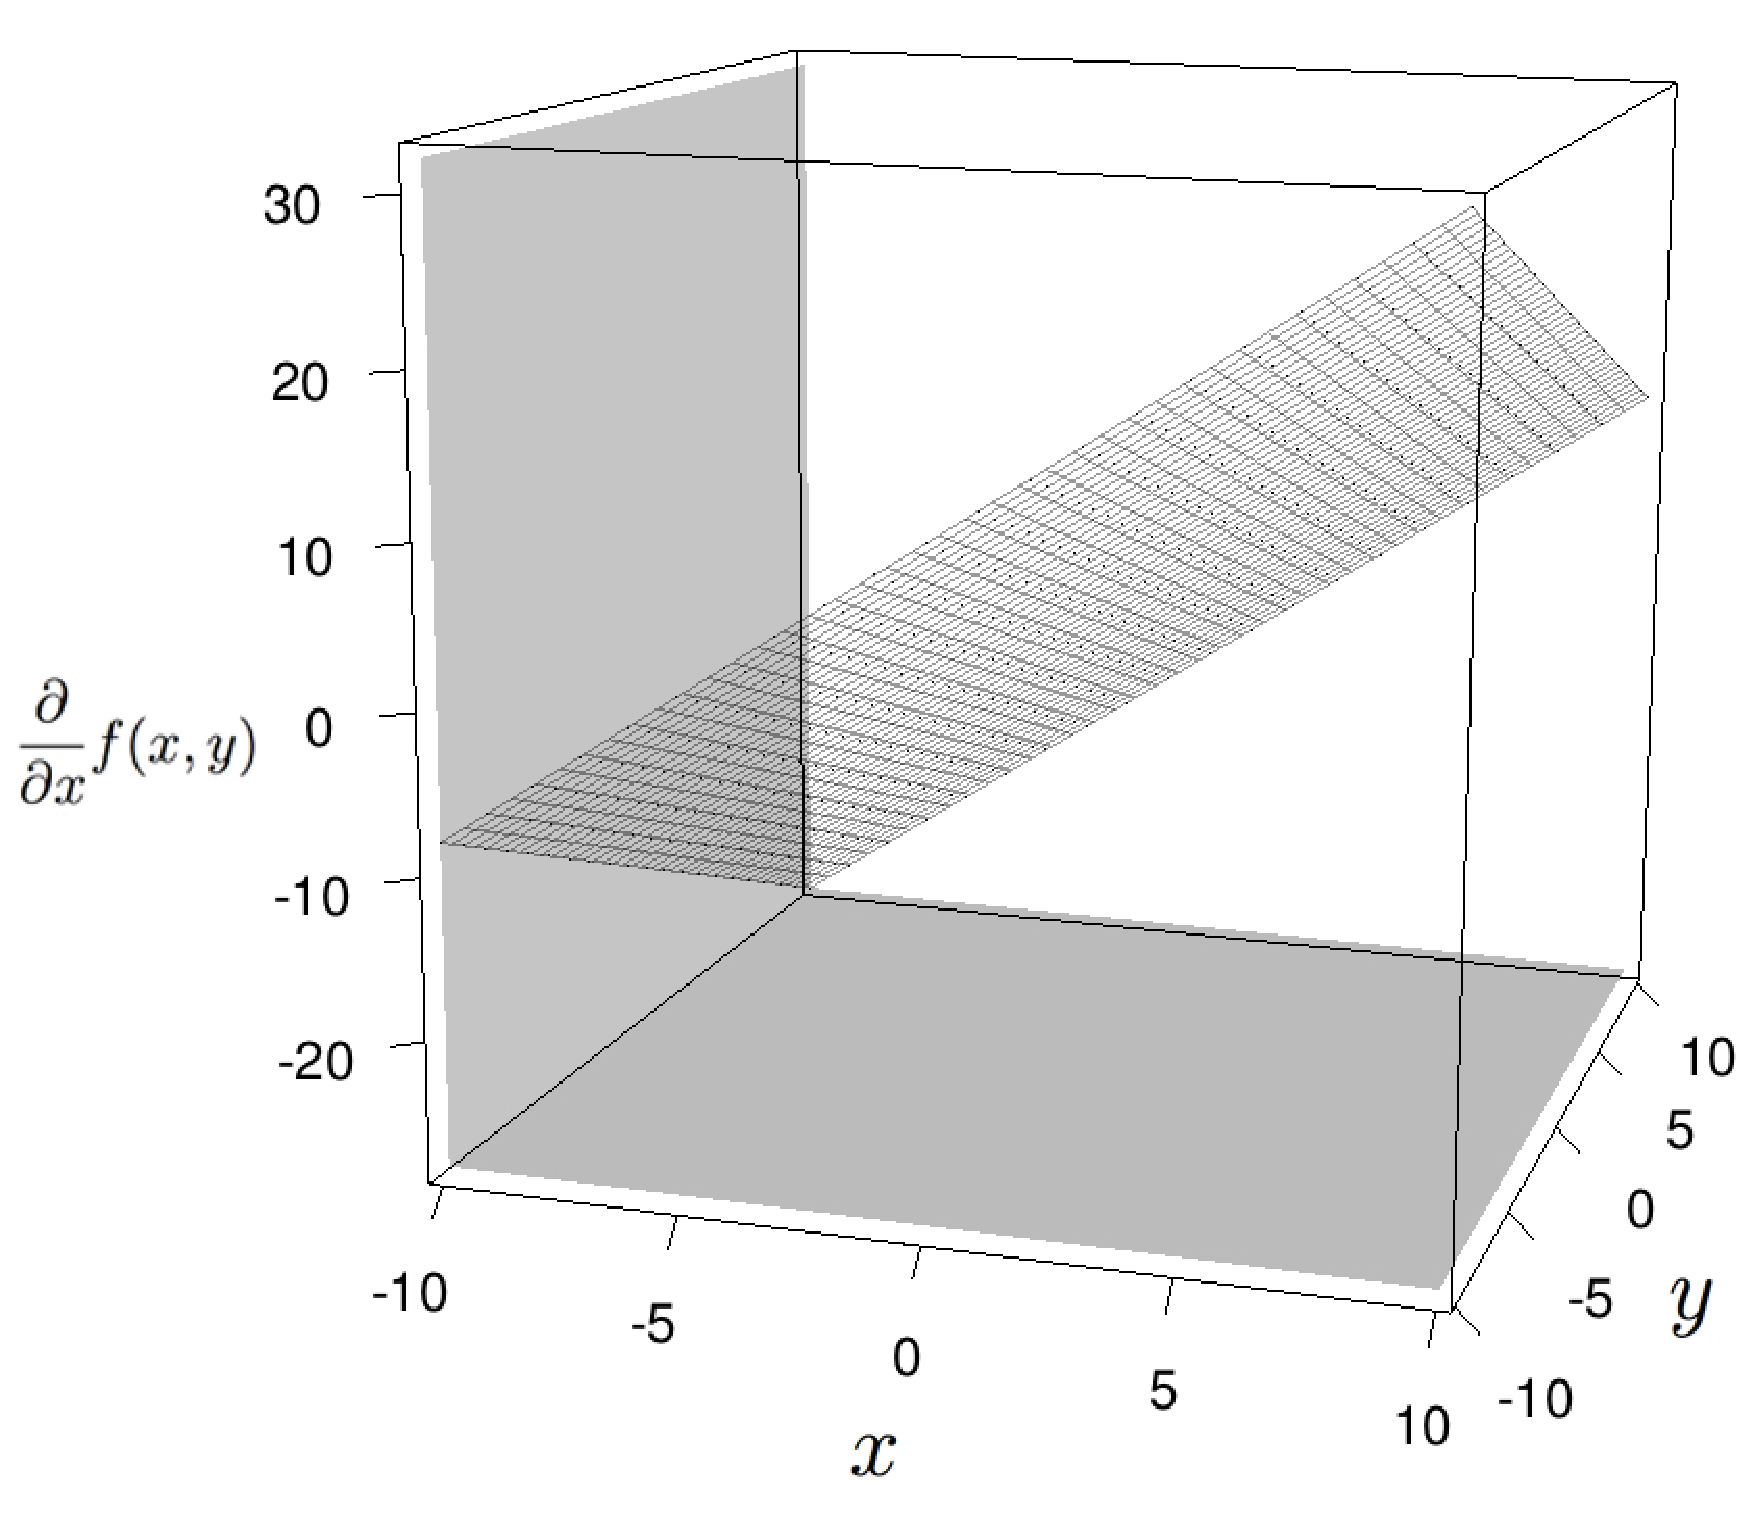
\includegraphics[width=0.32\textwidth]{./images/PartialDerivativesExampleX.pdf}}
\subfigure[$\displaystyle \frac{\partial}{\partial y} f(x, y) = -2y + 4 - x$]{\label{fig:partialDerivExample3}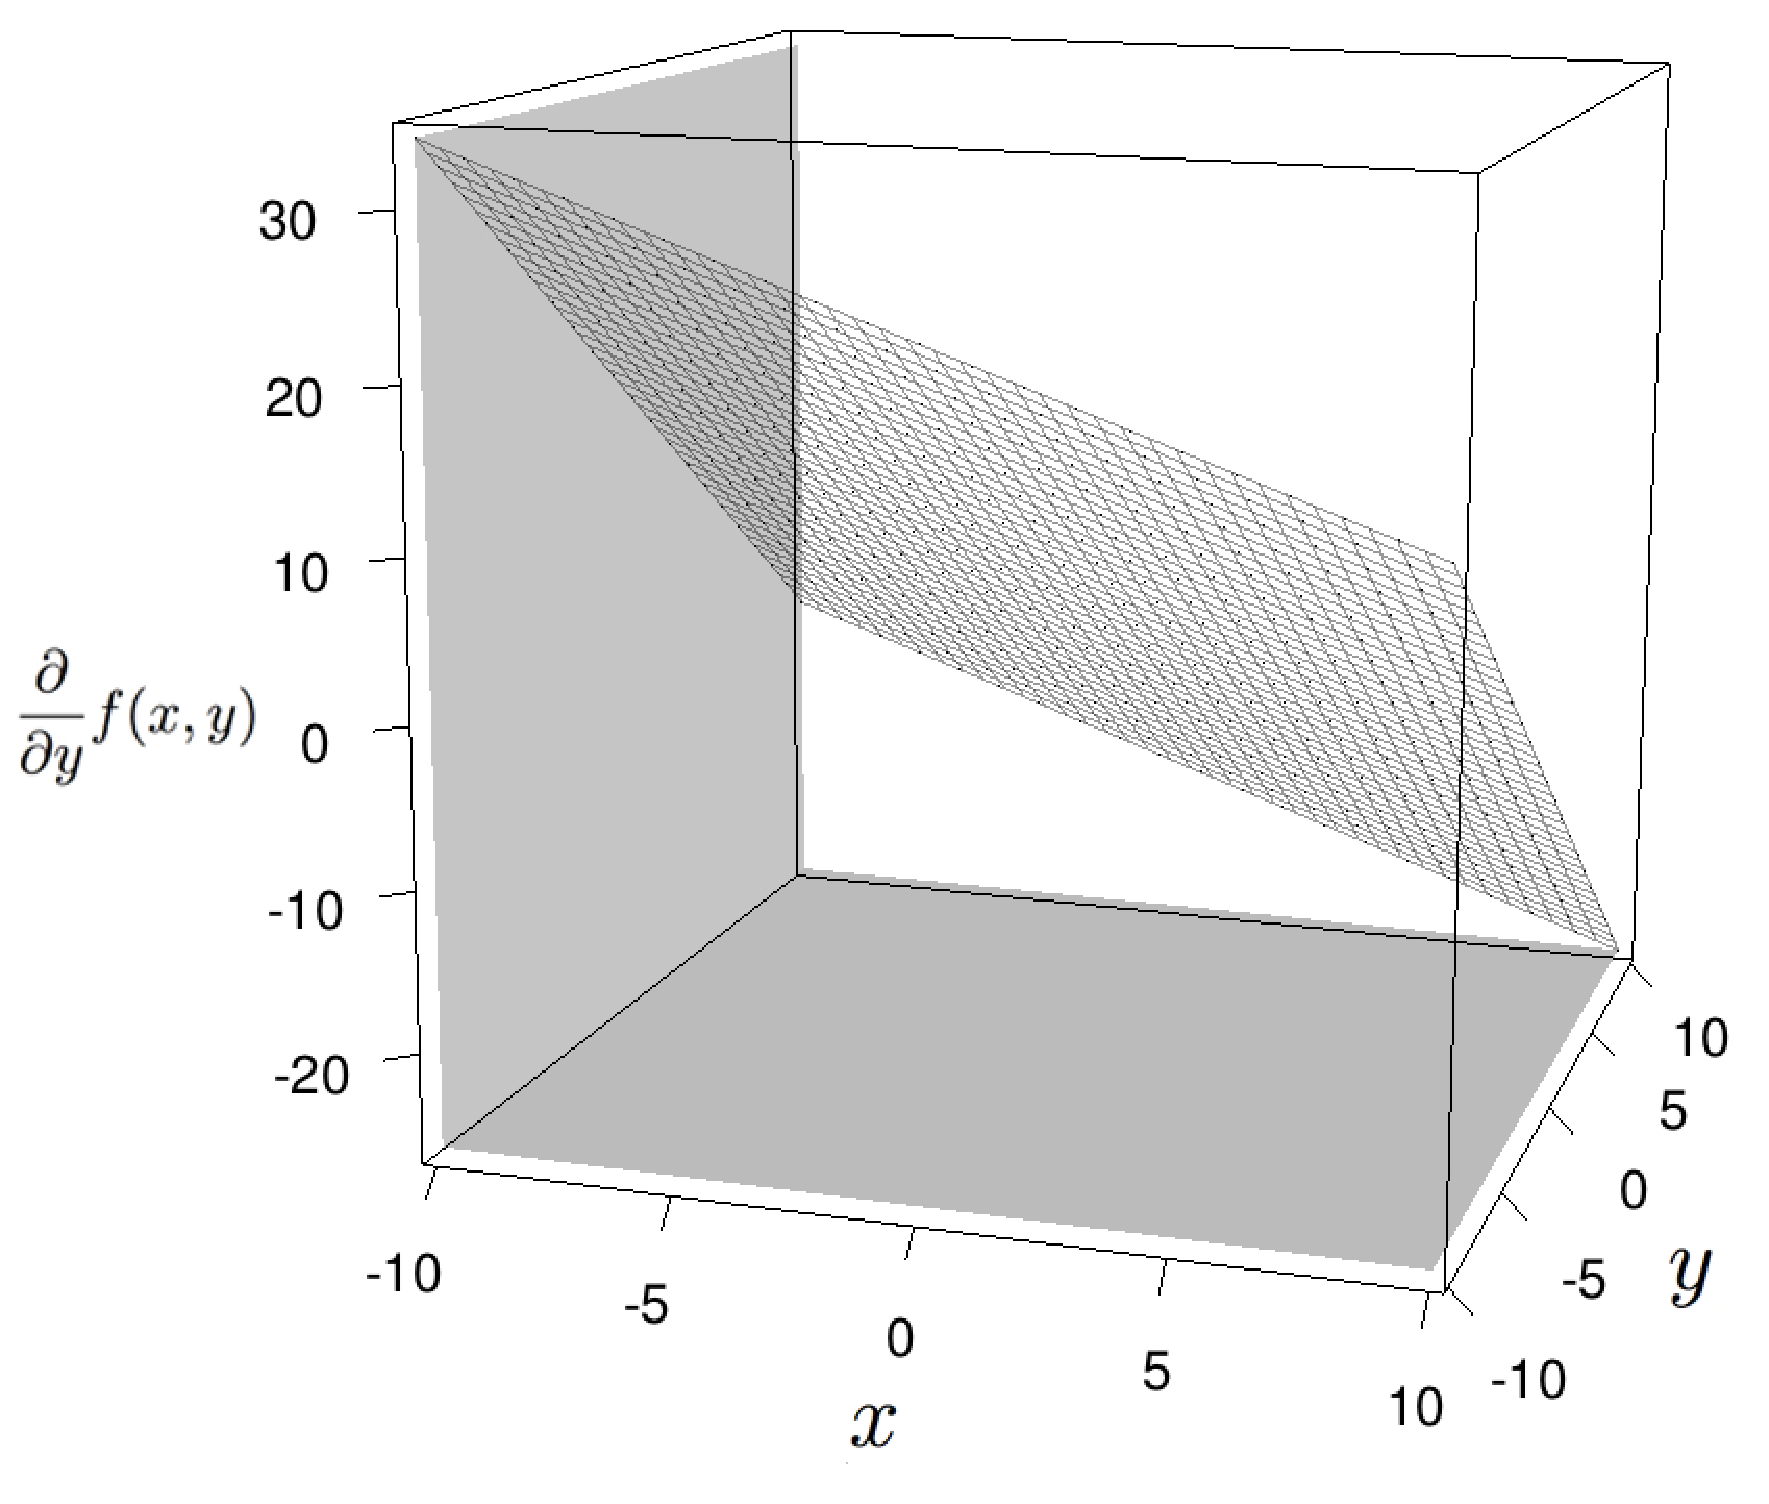
\includegraphics[width=0.32\textwidth]{./images/PartialDerivativesExampleY.pdf}}
\caption{(a) a continuous function in two variables, $x$ and $y$. (b) the partial derivative of this function with respect to $x$. (c) the partial derivative of this function with respect to $y$.}
\label{fig:partialDerivExample}
\end{center}
\end{figure}
\end{frame} 

\SectionSlide{Summary}

\begin{frame}
	\tableofcontents
\end{frame}

\end{document}
